\documentclass[10pt]{article}
\usepackage[colorlinks=true,linkcolor=black,urlcolor=black,citecolor=black]%
{hyperref}
\usepackage{cleveref}
\usepackage{cite}
\usepackage{calc}
\usepackage{ifthen}
\usepackage{tikz}

%adapted from http://www.texample.net/tikz/examples/pie-chart/
\newcommand{\slice}[3]{
  \draw[thick,fill=#3] (0,0) -- (#1:1) arc (#1:#2:1) -- cycle;
}

\title{The Next 700 Type Systems}
\author{Carlo Angiuli}
\date{March 31, 2017}

\begin{document}
\maketitle

Type systems classify programs in a way that enables compositional reasoning
about their behavior. As a result, type systems have found a place as one of the
major organizing principles of modern programming languages; much programming
language research focuses on new ways of classifying programs in order to
capture more sophisticated invariants, including dependent, gradual, refinement,
linear, intersection, and existential types.

However, I feel that modern type systems focus too narrowly on
\emph{classification}, which is but one of the twenty-one definitions of the
noun \emph{type} in the Oxford English Dictionary. This myopic view of types has
impeded the vast majority of the possible subdisciplines of type theory, as
depicted in \Cref{fig:pie-chart}.

\begin{figure}[b]
\centering
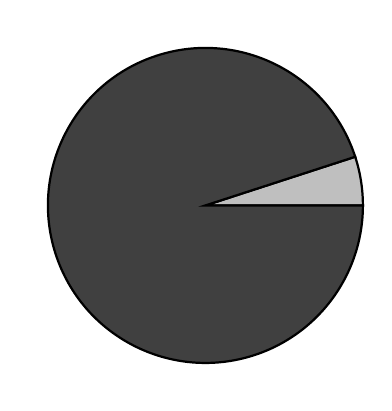
\begin{tikzpicture}[scale=2]
\slice{0}{5/100*360}{black!25}
\slice{5/100*360}{360}{black!75}
\end{tikzpicture}
\caption{95.2\% of the definitions of \emph{type, n.}, have not been explored in
the context of type systems.}
\label{fig:pie-chart}
\end{figure}

In the remainder of this paper, we describe a family of unimplemented type
systems that is intended to span differences of meaning by a group of disparate
frameworks \cite{landin66}.

\paragraph{The sort of person to whom one is attracted (\emph{one's type}).}

\paragraph{Tip.}

angels dancing on the head of a pin, cite Aquinas

\paragraph{Symbol, emblem}

\paragraph{A pattern stamped onto the face of a coin}

\paragraph{An imperial edict released by Emperor Constans II in AD 648
prohibiting arguments over the Christological doctrine of Monotheletism.}

\paragraph{An exemplar of a particular kind or order}

\paragraph{The specimen originally used to name a species (type specimen)}

\paragraph{A small block bearing a raised character, for use in printing}

\paragraph{Printed characters (in type)}

\paragraph{An abstract category, rather than its instantiations (type/token distinction)}

\paragraph{To write with a keyboard}

\bibliography{next}{}
\bibliographystyle{acm}

\end{document}
